\documentclass[aspectratio=169,10pt]{beamer}
\usepackage[T1]{fontenc}
\usepackage{lmodern}
\usepackage{graphicx,booktabs,amsmath}

\definecolor{ink}{HTML}{1f2933}
\definecolor{navy}{HTML}{3d5a80}
\definecolor{grey}{HTML}{7b8794}
\definecolor{orange}{HTML}{c0622f}

\setbeamertemplate{navigation symbols}{}
\setbeamercolor{normal text}{fg=ink}
\setbeamercolor{frametitle}{fg=ink}
\setbeamercolor{title}{fg=ink}
\setbeamercolor{subtitle}{fg=navy}
\setbeamerfont{frametitle}{series=\bfseries,size=\large}
\setbeamerfont{title}{series=\bfseries,size=\LARGE}
\setbeamertemplate{frametitle}{\vspace{0.6em}\insertframetitle}
\setbeamertemplate{footline}{\hfill\color{grey}\scriptsize\insertframenumber\hspace{1.2em}\vspace{0.8em}}
\setbeamertemplate{itemize items}{\color{navy}\textbullet}
\setbeamertemplate{enumerate items}{\color{navy}\insertenumlabel.}
\setbeamersize{text margin left=1.6em,text margin right=1.6em}

\newcommand{\hl}[1]{{\color{navy}\textbf{#1}}}
\newcommand{\bad}[1]{{\color{orange}#1}}
\newcommand{\refs}[1]{{\color{grey}\scriptsize #1}}
\newcommand{\lab}[1]{{\color{navy}\textbf{#1}}}
\newcommand{\bignum}[1]{{\color{navy}\fontsize{20}{22}\selectfont #1}}
\newcommand{\from}[1]{{\color{grey}\fontsize{13}{15}\selectfont #1}}

\title{Spectral normalization and truncation\\ on a fixed MLP GAN}
\subtitle{What each change adds to precision and recall on MNIST}
\author{Nourcène Brahem \quad Lukas Tabouri \quad Manel Wafra}
\date{DataLab A2, group 34 \quad·\quad 5 November 2026}

\begin{document}

% 1 ---------------------------------------------------------------------------
\begin{frame}[plain]
\vspace{2.6em}
{\usebeamerfont{title}\usebeamercolor[fg]{title}\inserttitle\par}
\vspace{0.6em}
{\large\color{navy}\insertsubtitle\par}
\vspace{2.6em}
{\color{grey}\insertauthor\par\vspace{0.3em}\insertdate}
\end{frame}

% 2 ---------------------------------------------------------------------------
\begin{frame}{Baseline: the starter code, unchanged}
\begin{columns}[c]
\column{0.5\textwidth}
\begin{itemize}\setlength\itemsep{0.8em}
\item BCE loss, Adam $\beta_1 = 0.9$\\ 100 epochs = 94k steps of $G$
\item \hl{3 seeds} for every configuration
\item FID, precision, recall on 10k samples,\\ computed as on the platform\\
 {\small\color{grey}(same checkpoint: 31.4 ours, 30.6 platform)}
\end{itemize}

\column{0.46\textwidth}
\centering
\begin{tabular}{@{}c@{\hspace{0.8em}}c@{}}
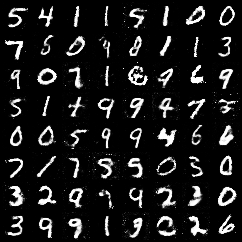
\includegraphics[width=0.44\linewidth]{g_starter_s0.png} &

\includegraphics[width=0.44\linewidth]{g_starter_s1.png}\\[0.1em]
{\scriptsize seed 0} & {\scriptsize\bad{seed 1: collapsed at epoch 2}}
\end{tabular}

\vspace{1.2em}
\begin{tabular}{@{}ccc@{}}
\bignum{29.5} & \bignum{0.49} & \bignum{0.24}\\
{\small FID} & {\small precision} & {\small recall}
\end{tabular}\\[0.3em]
{\scriptsize\color{grey}mean of the 2 seeds that train}
\end{columns}
\end{frame}

% 3 ---------------------------------------------------------------------------
\begin{frame}{One training change, one inference change}
\begin{columns}[T]
\column{0.47\textwidth}
\lab{Training: spectral normalization (SN)}\\[0.5em]
Each layer of $D$: \ $W \leftarrow W / \sigma_{\max}(W)$\\[0.3em]
With the setting of the paper:\\ hinge loss, Adam $\beta_1 = 0.5$, 5 $D$ steps per $G$ step\\[1.2em]
\hl{H1}\enspace more stable training, higher recall

\column{0.47\textwidth}
\lab{Inference: truncation vs.\ rejection}\\[0.5em]
\textbf{Truncation}: resample $z_i$ until $|z_i| \le \psi$\\
{\small\color{grey}cost $1\times$}\\[0.3em]
\textbf{DRS}: keep $x$ with a probability given by $D(x)$\\
{\small\color{grey}cost $K = 5\times$, $D$ retrained 3 epochs with $G$ frozen}\\[0.6em]
\hl{H2}\enspace both raise precision,\\ only truncation loses recall
\end{columns}

\vfill
\refs{SN: Miyato et al., ICLR 2018 \quad·\quad Truncation: Brock et al.\ (BigGAN), ICLR 2019 \quad·\quad
DRS: Azadi et al., ICLR 2019}
\vspace{0.4em}
\end{frame}

% 4 ---------------------------------------------------------------------------
\begin{frame}{Training: SN only catches up, at 6$\times$ the time}
\centering
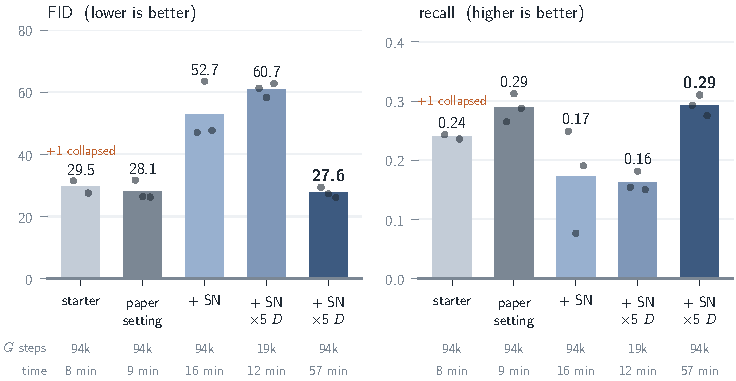
\includegraphics[width=0.74\textwidth]{s_train.pdf}

\vspace{0.6em}
\begin{columns}[T]
\column{0.92\textwidth}
\begin{itemize}\setlength\itemsep{0.2em}\small
\item The paper setting alone removes the collapse and raises recall \textbf{0.24 $\to$ 0.29}
\item SN needs 5 $D$ steps per $G$ step to match it \quad{\small\color{grey}(with the starter loss: FID 177)}
\item \hl{H1}: stability yes, extra recall from SN no
\end{itemize}
\end{columns}
\end{frame}

% 5 ---------------------------------------------------------------------------
\begin{frame}{Inference: SN keeps its recall under truncation}
\centering
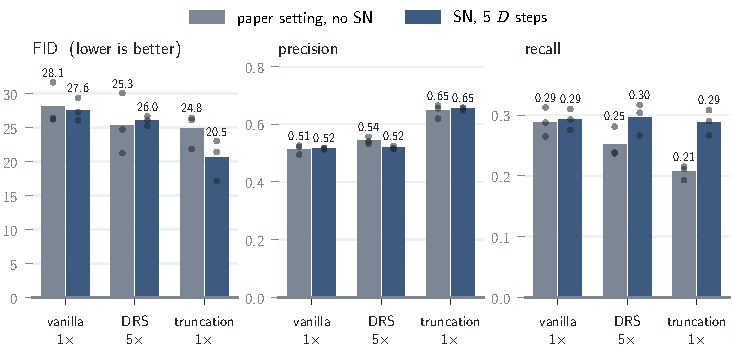
\includegraphics[width=0.74\textwidth]{s_inf.pdf}

\vspace{0.6em}
\begin{columns}[T]
\column{0.92\textwidth}
\begin{itemize}\setlength\itemsep{0.2em}\small
\item Truncation $\psi = 1$: precision \textbf{0.52 $\to$ 0.65} for both models,
 recall kept \textbf{only with SN} {\small\color{grey}(3/3 seeds)}
\item DRS: small gain, 5$\times$ the samples
\item \hl{H2}: rejected, free truncation beats rejection here
\end{itemize}
\end{columns}
\end{frame}

% 6 ---------------------------------------------------------------------------
\begin{frame}{Result and limits}
\begin{columns}[T]
\column{0.5\textwidth}
\lab{Starter baseline $\to$ SN + truncation}\\[0.2em]
{\scriptsize\color{grey}mean over 3 seeds}\\[0.8em]
\begin{tabular}{@{}l@{\hspace{1em}}r@{\hspace{0.6em}}c@{\hspace{0.6em}}l@{}}
FID & \from{29.5} & $\to$ & \bignum{20.5}\\[0.5em]
precision & \from{0.49} & $\to$ & \bignum{0.65}\\[0.5em]
recall & \from{0.24} & $\to$ & \bignum{0.29}
\end{tabular}

\vspace{1em}
{\small Recall: from the training setting.\\ Precision: from truncation, which SN makes safe.}

\column{0.46\textwidth}
\lab{Limits}\\[0.5em]
\begin{itemize}\setlength\itemsep{0.6em}
\item 3 seeds: gaps under 3 FID are noise
\item $\psi$ chosen on the reported metrics
\item 5 $D$ steps never tested without SN
\item Why SN helps truncation: not explained yet
\end{itemize}
\end{columns}
\end{frame}

% 7 ---------------------------------------------------------------------------
\begin{frame}{Next steps}
\begin{enumerate}\setlength\itemsep{1.0em}
\item Paper setting with 5 $D$ steps \textbf{without} SN: the missing ablation
\item SN + TTUR instead of 5 $D$ steps: same effect, without $6\times$ the time?
\item OBRS: rejection with an optimal budget, against truncation at equal cost
\item Choose $\psi$ on a held-out split; measure how smooth $G$ is with and without SN
\end{enumerate}

\vfill
\refs{TTUR: Heusel et al., NeurIPS 2017 \quad·\quad OBRS: Vérine et al., AISTATS 2024}
\vspace{0.4em}
\end{frame}

\end{document}
